% Drawing 79/02-2 -- folder 79, batch 02, archive page 32 (PDF page 33).
% Transcription: losange de sommets $u$ (en haut), $s$ (à gauche), $t$ (à droite), $u'$ (en bas), coupé par la diagonale $a = st$ ; dans la face supérieure $f$, le drapeau hachuré $r$ et ses voisins $\tau_1 r$, $\tau_0 r$, $\tau_\infty r$, ce dernier passant dans la face inférieure.
% Kind: rhombus of two triangles with a flag and its neighbours. Method 2 (schematic redraw from the facsimile). Status: ok.
% Notes: Rhombus u (top), s (left), t (right), u' (bottom) cut by the diagonal a = st. In the upper face f the hatched flag r at s and its neighbours tau_1 r, tau_0 r; tau_infty r below the diagonal, in the lower face. Label a sits in the lower face, under the diagonal.
% Coordinates: 1 unit = 1 mm = 1/100 of the crop width (bbox in page fractions: [0.2, 0.08, 0.34, 0.23]).
% Redrawn by Claude (claude-opus-5-5), issue #73, 2026-11-07; not checked by a human; not compiled (no TeX in the session).
% Rights: reproduces part of the work -- behind RENDER_TRANSCRIPTS, never published by itself.
\documentclass[tikz,border=3pt]{standalone}
\usepackage{amsmath,amssymb}
\usetikzlibrary{patterns,arrows.meta}
\tikzset{pencil/.style={black!45}, struck/.style={black!35}, mark/.style={circle,draw,inner sep=1.3pt}, pt/.style={circle,fill,inner sep=0.9pt}, opt/.style={circle,draw,fill=white,inner sep=1.1pt}}
\begin{document}
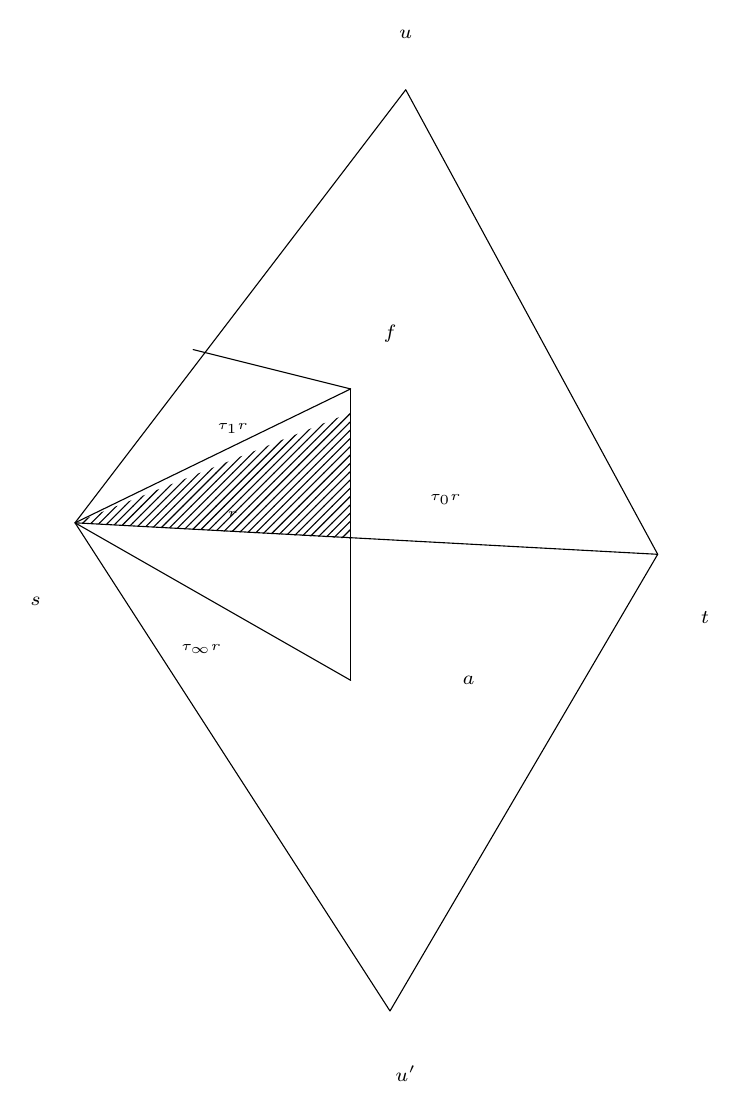
\begin{tikzpicture}[x=1mm,y=1mm,line cap=round,line join=round,font=\scriptsize]
\draw (52,-25) -- (84,-84) -- (50,-142) -- (10,-80) -- cycle;
\draw (10,-80) -- (84,-84);
\draw (10,-80) -- (45,-63);
\draw (45,-63) -- (45,-100);
\draw (45,-100) -- (10,-80);
\fill[pattern=north east lines] (10,-80) -- (45,-66) -- (45,-82) -- cycle;
\draw (25,-58) -- (45,-63);
\node[inner sep=1pt] at (52,-18) {\scriptsize $u$};
\node[inner sep=1pt] at (5,-90) {\scriptsize $s$};
\node[inner sep=1pt] at (90,-92) {\scriptsize $t$};
\node[inner sep=1pt] at (52,-150) {\scriptsize $u'$};
\node[inner sep=1pt] at (50,-56) {\scriptsize $f$};
\node[inner sep=1pt] at (30,-68) {\tiny $\tau_1 r$};
\node[inner sep=1pt] at (30,-79) {\tiny $r$};
\node[inner sep=1pt] at (57,-77) {\tiny $\tau_0 r$};
\node[inner sep=1pt] at (26,-96) {\tiny $\tau_\infty r$};
\node[inner sep=1pt] at (60,-100) {\scriptsize $a$};
\end{tikzpicture}
\end{document}
